\documentclass[a4paper, 12pt]{article}
\usepackage[utf8]{inputenc}
\usepackage[english,russian]{babel}
\usepackage[warn]{mathtext}
\usepackage{graphicx}
\usepackage{float}
\usepackage{multirow}
\restylefloat{table}
\usepackage{amsmath}
\usepackage{floatflt}
\usepackage[T2A]{fontenc}
\usepackage[left=20mm, top=20mm, right=20mm, bottom=20mm, footskip=10mm]{geometry}

\tolerance 1414
\hbadness 1414
\emergencystretch 1.5em
\hfuzz 0.3pt        % размер максимального переполнения без warning'a
\widowpenalty=10000 % запрещает одиночную строку абзаца в начале страницы
\vfuzz \hfuzz
\raggedbottom       % если на странице мало содержимого, добавить пустое место в конце, а не в середине страницы



\begin{document}

\begin{titlepage}
	\centering
	\vspace{5cm}
	{\scshape\LARGE московский физико-технический институт (национальный исследовательский университет) \par}
	\vspace{6cm}
	{\scshape\Large Лабораторная работа 4.7.3 \par}
	{\huge\bfseries Поляризация света \par}
	\vspace{1cm}
	\vfill
\begin{flushright}
	{\large Б03-102}\par
	\vspace{0.3cm}
	{\LARGE Куланов Александр}
\end{flushright}
	

	\vfill


	Долгопрудный, 2023 г.
\end{titlepage}

\begin{itemize}
	\item \textbf{Цель работы:} изучение зависимости показателя преломления необыкновенной волны от направления в двоякопреломляющем кристалле; определение главных показателей преломления $n_o$ -- обыкновенной и $n_e$ -- необыкновенной волны в кристалле; наблюдение эффекта полного внутреннего отражения
    \item \textbf{В работе используются:} лазерная указка, вращающийся сотолик с неподвижным лимбом, призма из исландского шпата, поляроид.
\end{itemize}

\section{Экспериментальная установка}

\section{Теоретические сведения}

\subsection*{Плоские волны в кристаллах}
\begin{equation}
\text{rot} \vec{H} = \dfrac{1}{c}\dfrac{\partial \vec{D}}{\partial t}, \text{rot} \vec{E} = -\dfrac{1}{c}\dfrac{\partial \vec{B}}{\partial t}
\end{equation}
Если среды прозрачны и однородны то в них распорстраняются волны:
\begin{equation}
\vec E = \vec{E}_0 e^{i(\omega t - \vec{k}\vec{r})}, \vec{H} = \vec{H}_0e^{i(\omega t - \vec{k}\vec{r})}
\end{equation}
Введем единичный вектор нормали к скорости распространения волны $\vec{N}$ и направим его вдоль скорости, тогда
\begin{equation}
\vec{D} = -\dfrac{c}{v}\left[\vec{N}, \vec{H}\right], \vec{B} = \dfrac{c}{v}\left[	\vec{N}, \vec{E}\right]
\end{equation}
\subsection*{Оптические одноосные кристаллы}
Введем \textit{тензор диэлектрической проницаемости} $\varepsilon$ ($\vec{D} = \varepsilon \vec{E}$). Все его значения описываются эллипсоидом инерции. 

В кристаллах этот эллипсоид --- эллипсоид вращения. В них оптическая ось --- ось вращения эллипсоида. В них принято обозначать $\varepsilon_{\parallel} = \varepsilon_z, \varepsilon_{\perp} = \varepsilon_x = \varepsilon_y$

\begin{equation}
\vec{D}_{\parallel} = \varepsilon_{\parallel} \vec{E}_{\parallel},\vec{D}_{\perp} = \varepsilon_{\perp} \vec{E}_{\perp} 
\end{equation}

Можно показать, что угол $\theta$ между волновой нормалью и осью вращения эллипсоида при разделении $\vec{D}$ на $\vec{D}_e$ --- лежащая в главном сечении и $\vec{D}_o$ --- нормальная составляющая такой, что
\begin{equation}
\sin \theta = \dfrac{D_{e\parallel}}{D_e}, \cos \theta = \dfrac{D_{e\perp}}{D_e}
\end{equation}
\begin{equation}
n = \dfrac{1}{\sin A}\sqrt{\sin^2 \phi_1 + \sin^2 \phi_2 + 2 \sin \phi_1 \sin \phi_2 \cos A}
\end{equation}
Из этого, если $n_o - n_e \ll n_o$ и $n_e$, то 
\begin{equation}
n(\theta) \approx n_e + (n_o - n_e) \cos^2 \theta
\end{equation}
%\newpage
\subsection*{Двойное лучепреломление в призме исландского шпата}
\begin{figure}
	\begin{center}
		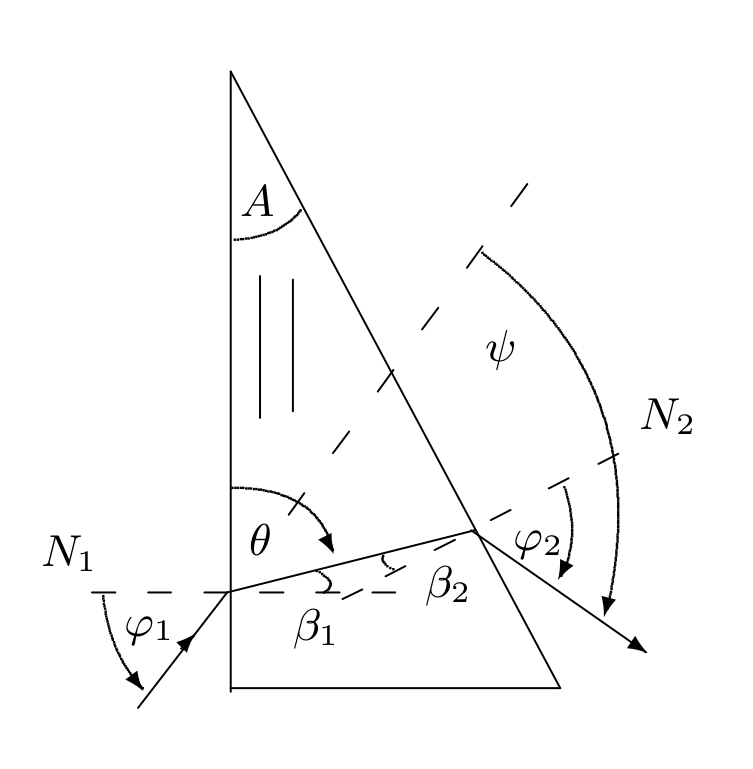
\includegraphics[width = 0.5\textwidth]{prism.png}
		  \end{center}
	  \caption{Ход луча в призме}
\end{figure}
При таком ходе луча и расположении призмы у нас повторяется ситуация из предыдущего параграфа теории. Тогда, можно посчитать показатель преломления изотропной среды по формуле 
\begin{equation}
n = \dfrac{\sin\left(\dfrac{\psi_m + A}{2}\right)}{\sin \left(\dfrac{A}{2}\right)}
\end{equation}
Здесь $\psi_m$  --- минимальный угол, на который призма преломляет луч.
Если призма неизотропна, то этой формулой, строго говоря, можно воспользоваться только для обыкновенной волны, которая, как это было показано ранее, распространяется так же, как и в изотропной среде. 

\end{document}